\documentclass[11pt]{article}
\usepackage[utf8]{inputenc}
\usepackage[T1]{fontenc}
\usepackage[english]{babel}
\usepackage{geometry}
\geometry{a4paper, top=2.5cm, bottom=2.5cm, left=3cm, right=3cm}
\usepackage{array}
\usepackage{float}
\usepackage{placeins}
\usepackage{csvsimple}
\usepackage{longtable}



\usepackage{amsmath}

\newcommand{\hardswish}{\operatorname{h-swish}}
\newcommand{\relu}{\operatorname{ReLU}}
\newcommand{\sigmoid}{\operatorname{\sigma}}

% big tick = main responsible person, small tick = supporting team member
\newcommand{\mainresp}{{\LARGE$\checkmark$}}
\newcommand{\suppresp}{{\footnotesize$\checkmark$}}

\usepackage[backend=bibtex, style=ieee]{biblatex}
%\addbibresource{bibliography.bib}

\usepackage{caption}
\usepackage{subcaption}

\usepackage{booktabs}
\usepackage{graphicx}
\usepackage{amssymb}
\usepackage{multirow}
\usepackage{tikz}
\usetikzlibrary{shapes.geometric, arrows.meta}

% stick figure actor for use case diagrams: #1 = node name, #2 = position, #3 = label
\newcommand{\actor}[3]{
    \begin{scope}[shift={(#2)}]
        \draw (0,0.95) circle (0.2);
        \draw (0,0.75) -- (0,0.2);
        \draw (-0.35,0.55) -- (0.35,0.55);
        \draw (0,0.2) -- (-0.25,-0.25);
        \draw (0,0.2) -- (0.25,-0.25);
        \node[below, align=center] at (0,-0.3) {#3};
        \node[inner sep=0pt, minimum width=0.8cm, minimum height=1.5cm] (#1) at (0,0.4) {};
    \end{scope}
}

\title{
    \textbf{Big Data Solution for Warsaw Public Transit delay prediction - Milestone 2 report} \\[0.5cm]
    \large Big Data Analytics
}
\author{Emil Łasocha \and Michał Szewczak \and Sebastian Trojan \and Tymoteusz Urban}
\date{\today}

\begin{document}

\maketitle
% \newpage

\section{Updates to PM1 Report}

The main business and technical assumptions presented in PM1 remain unchanged. However, three modifications were introduced during implementation:

\subsection{Data Sources}
\label{sec:updates-data-sources}

GPS and GTFS data sources were changed from the Warsaw Open Data API to mkuran.pl. Weather and air quality data are still taken from the Warsaw Open Data API. Unlike the original API, mkuran.pl provides \texttt{trip\_id} and \texttt{service\_date} alongside GPS observations, as well as ready-to-use GTFS files. This simplifies matching vehicle positions to scheduled trips and calculating delays, as identifying the correct trip for each vehicle independently would require a complex matching process based on location, time, and timetable data.

\subsection{Removal of Hive Metastore}

Hive Metastore was removed from the architecture, as Apache Spark can directly read and process Parquet files stored in HDFS. This simplifies the infrastructure and eliminates the need to maintain an additional service.

\subsection{Simulation Buffering}

The buffering period was increased from 10 to 15 minutes. Analysis of the weather and air quality APIs showed that although measurements have timestamps at 10-minute intervals, new data is not published simultaneously for all stations. Update delays vary between stations, and new measurements are not always available every 10 minutes. The longer buffer increases the likelihood that the necessary measurements will be available for proper synchronisation and interpolation before the simulated data is published.
\section{Description}

The goal of the project is to build a system that shows current delays in Warsaw's public transport, how they will change in the near future, and how these delays depend on weather and air conditions. The system will collect live positions of buses and trams, timetables, weather data and air quality data published by the city. By comparing the real position of a vehicle with its timetable we can calculate its delay. Then this information is combined with current weather and used both for live monitoring and for training a machine learning model that predicts delays.

Weather is an obvious candidate for a factor that affects delays, because rain, snow or ice make traffic slower. Air quality is less obvious, but we expect some correlation with delays, since heavy traffic both slows down buses and makes the air quality worse. One of the goals of the project is to check how strong these relations really are.

From the user perspective, the final product is a web dashboard which presents current delays, predicted delays and historical statistics in a simple form.

\section{Project Deliverables and Users}

\subsection{Target users}

We identified three main groups of users of the system:
\begin{itemize}
    \item \textbf{Passenger} - a person who travels by bus or tram in Warsaw and wants to know if their line is on time and what delay to expect, especially in bad weather.
    \item \textbf{Dispatcher} - a person working for the transport operator who watches the whole network during the day and needs to react quickly when delays start to grow.
    \item \textbf{Transport planner / analyst} - a person who works on timetables and the transport network in the long term and wants to understand where and why delays appear.
\end{itemize}

\subsection{Deliverables}

After finishing the project, the users will get access to the following features:
\begin{itemize}
    \item \textbf{Live delay monitoring} - current position and delay of vehicles, which can be filtered by line or stop, and a map of the network with delays marked on it. Next to the delay information, the dashboard also shows current weather and air quality measured by stations located in the city.
    \item \textbf{Delay prediction} - predicted delay of a given line at a given stop for the near future, calculated by a machine learning model working on streaming data and taking into account current weather and air quality. Based on the predictions, the dashboard also shows alerts with a list of lines and areas where the predicted delay is higher than a chosen threshold, so problems can be noticed beforehand.
    \item \textbf{Historical statistics and weather impact analysis} - average delays by line, stop, hour of the day, day of the week and weather conditions, calculated with batch processing on all collected data. This also includes a comparison of delays in different weather conditions (for example dry vs. rainy days) and a list of lines and stops which are most sensitive to bad weather.
\end{itemize}

\subsection{Use cases}

The use case diagram of the system is presented in Figure~\ref{fig:use_cases}.

\begin{figure}[H]
\centering
\resizebox{\textwidth}{!}{%
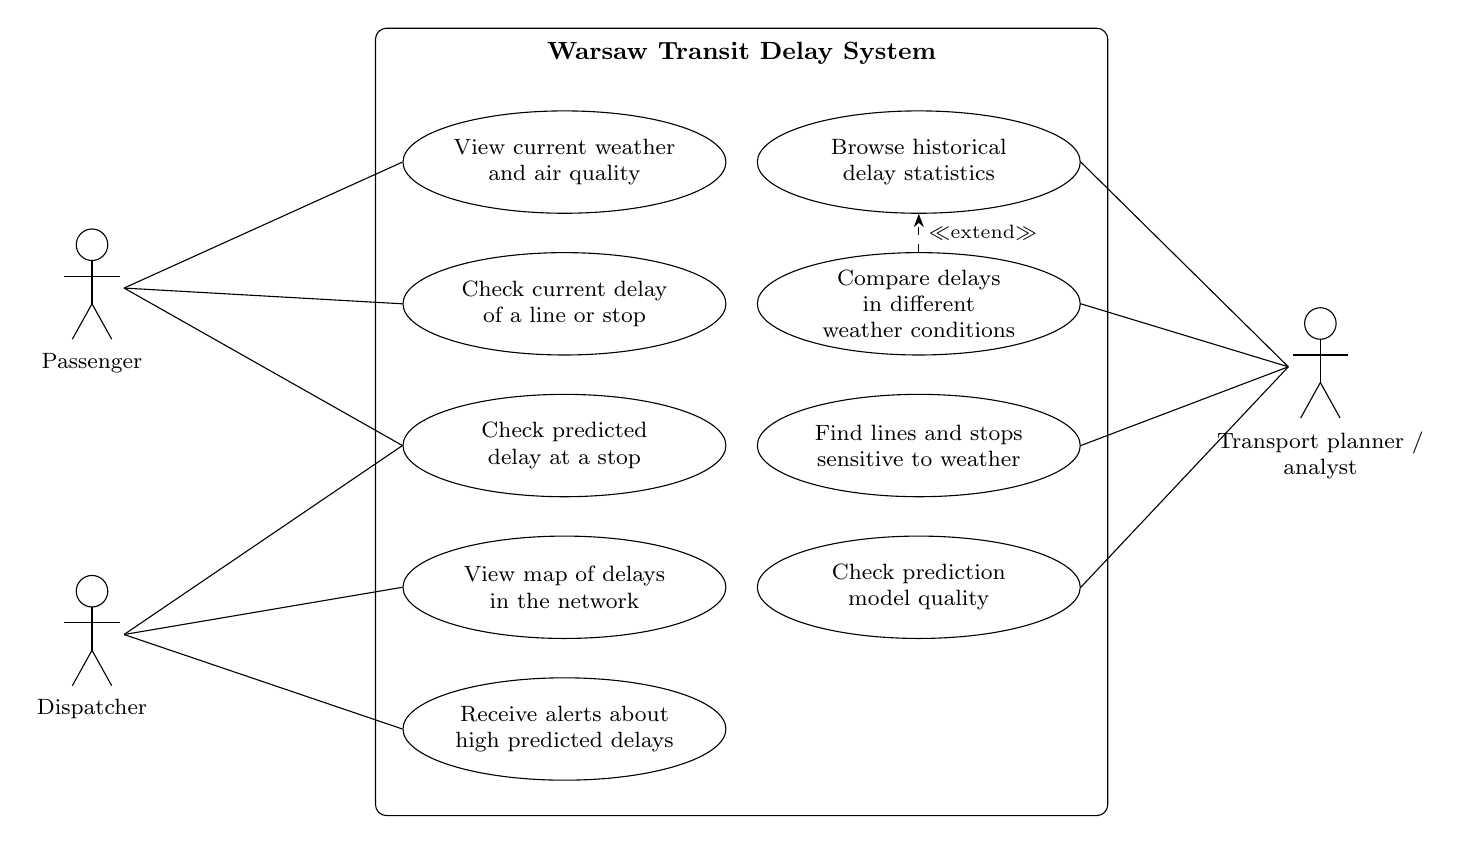
\begin{tikzpicture}[
    usecase/.style={draw, ellipse, inner sep=0pt, minimum width=4cm, minimum height=1.3cm, text width=2.9cm, align=center, font=\footnotesize, execute at begin node={\hyphenpenalty=10000}},
    assoc/.style={thin},
    every node/.append style={font=\footnotesize}
]
    % system boundary
    \draw[rounded corners] (3.6,3.7) rectangle (12.9,13.7);
    \node[anchor=north, font=\small\bfseries] at (8.25,13.65) {Warsaw Transit Delay System};

    % use cases for passengers and dispatchers
    \node[usecase] (uc3) at (6,12) {View current weather and air quality};
    \node[usecase] (uc1) at (6,10.2) {Check current delay of a line or stop};
    \node[usecase] (uc2) at (6,8.4) {Check predicted delay at a stop};
    \node[usecase] (uc4) at (6,6.6) {View map of delays in the network};
    \node[usecase] (uc5) at (6,4.8) {Receive alerts about high predicted delays};

    % use cases for planners
    \node[usecase] (uc6) at (10.5,12) {Browse historical delay statistics};
    \node[usecase] (uc7) at (10.5,10.2) {Compare delays in different weather conditions};
    \node[usecase] (uc8) at (10.5,8.4) {Find lines and stops sensitive to weather};
    \node[usecase] (uc9) at (10.5,6.6) {Check prediction model quality};

    % actors
    \actor{pas}{0,10}{Passenger}
    \actor{dis}{0,5.6}{Dispatcher}
    \actor{pla}{15.6,9}{Transport planner /\\ analyst}

    % associations
    \draw[assoc] (pas.east) -- (uc3.west);
    \draw[assoc] (pas.east) -- (uc1.west);
    \draw[assoc] (pas.east) -- (uc2.west);
    \draw[assoc] (dis.east) -- (uc2.west);
    \draw[assoc] (dis.east) -- (uc4.west);
    \draw[assoc] (dis.east) -- (uc5.west);
    \draw[assoc] (pla.west) -- (uc6.east);
    \draw[assoc] (pla.west) -- (uc7.east);
    \draw[assoc] (pla.west) -- (uc8.east);
    \draw[assoc] (pla.west) -- (uc9.east);

    % extend relation
    \draw[dashed, -{Stealth}] (uc7.north) -- node[right, font=\scriptsize] {$\ll$extend$\gg$} (uc6.south);
\end{tikzpicture}%
}
\caption{Use case diagram of the system}
\label{fig:use_cases}
\end{figure}

% \begin{table}[!t]
% \centering
% \caption{Description of use cases}
% \label{tab:use_cases}
% \small
% \begin{tabular}{>{\raggedright\arraybackslash}p{0.06\textwidth} >{\raggedright\arraybackslash}p{0.22\textwidth} >{\raggedright\arraybackslash}p{0.14\textwidth} >{\raggedright\arraybackslash}p{0.46\textwidth}}
% \toprule
% \textbf{ID} & \textbf{Name} & \textbf{Actor} & \textbf{Description} \\
% \midrule
% UC1 & Check current delay of a line or stop & Passenger & The user selects a line or a stop and sees the current delay of vehicles, calculated from live GPS data and the timetable. \\
% UC2 & Check predicted delay at a stop & Passenger, Dispatcher & The user selects a line and a stop and gets a predicted delay for the near future, generated by the ML model using live transit and weather data. \\
% UC3 & View current weather and air quality & Passenger & The user sees current temperature, precipitation, wind, visibility and air quality in different parts of the city. \\
% UC4 & View map of delays in the network & Dispatcher & The user sees a map with current vehicle positions coloured by their delay, which helps to quickly find problematic areas. \\
% UC5 & Receive alerts about high predicted delays & Dispatcher & The dashboard shows a list of lines where the predicted delay is above a chosen threshold. \\
% UC6 & Browse historical delay statistics & Planner & The user browses average delays by line, stop, hour and day of the week, calculated in batch mode on all collected data. \\
% UC7 & Compare delays in different weather conditions & Planner & An extension of UC6, where the user filters the statistics by weather conditions (e.g. rain, snow, low temperature) and compares the results. \\
% UC8 & Find lines and stops sensitive to weather & Planner & The user gets a ranking of lines and stops where delays grow the most in bad weather. \\
% UC9 & Check prediction model quality & Planner & The user sees evaluation metrics of the model (e.g. mean absolute error of predicted delay) and how they change over time. \\
% \bottomrule
% \end{tabular}
% \end{table}

\FloatBarrier
\subsection{Business process diagrams}

Figures~\ref{fig:bp_passenger} and~\ref{fig:bp_dispatcher} show the two core business processes of the system. The first one describes a passenger who checks the delay of their line before a trip. The second one describes a dispatcher who monitors delays in the whole network. Both processes end with a decision made by the user based on the data from the dashboard. The passenger can go to the stop as planned when the delay is small. When the current delay is big, the vehicle will simply arrive later, so the passenger can stay at home and go to the stop later. When the predicted delay is big, the situation on the route is expected to get worse, so the passenger can choose another line or other means of transport. The dispatcher can send a reserve vehicle when the problem affects one line, inform passengers and drivers when delays appear on many lines (for example because of bad weather), or take no action and keep monitoring. These actions are done by the users themselves, so our system only gives them the information needed to make the decision.

\begin{figure}[!htbp]
\centering
\resizebox{\textwidth}{!}{%
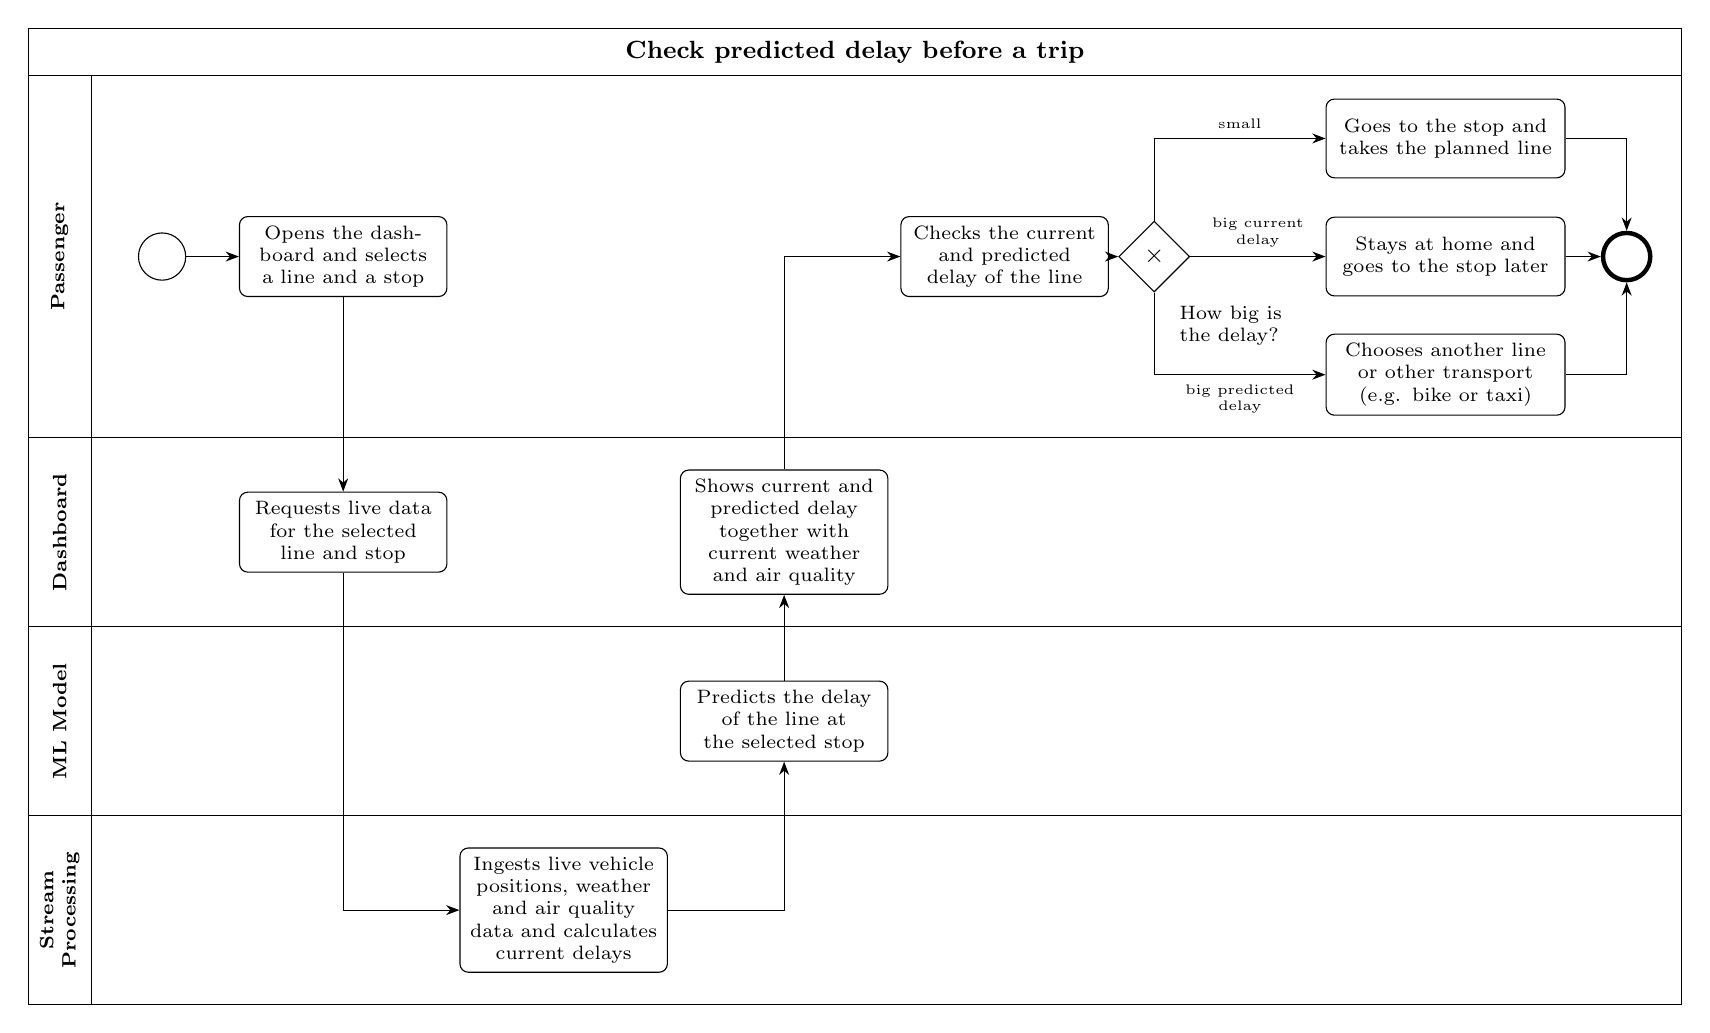
\begin{tikzpicture}[
    task/.style={draw, rounded corners=3pt, text width=2.4cm, minimum height=1cm, align=center, font=\scriptsize, fill=white},
    choice/.style={task, text width=2.8cm},
    event/.style={draw, circle, minimum size=0.6cm, inner sep=0pt, fill=white},
    endevent/.style={event, line width=1.6pt},
    gateway/.style={draw, diamond, minimum size=0.9cm, inner sep=0pt, fill=white, font=\small},
    flow/.style={-{Stealth}, thin},
    lane/.style={font=\scriptsize\bfseries, rotate=90}
]
    % pool and lanes
    \draw (0,0) rectangle (21,12.4);
    \draw (0,11.8) -- (21,11.8);
    \node[font=\small\bfseries] at (10.5,12.1) {Check predicted delay before a trip};
    \draw (0.8,0) -- (0.8,11.8);
    \foreach \y in {2.4,4.8,7.2} \draw (0,\y) -- (21,\y);
    \node[lane] at (0.4,9.5) {Passenger};
    \node[lane] at (0.4,6.0) {Dashboard};
    \node[lane] at (0.4,3.6) {ML Model};
    \node[lane, align=center] at (0.4,1.2) {Stream\\Processing};

    % elements
    \node[event] (s) at (1.7,9.5) {};
    \node[task] (p1) at (4,9.5) {Opens the dashboard and selects a line and a stop};
    \node[task] (p2) at (4,6.0) {Requests live data for the selected line and stop};
    \node[task] (p3) at (6.8,1.2) {Ingests live vehicle positions, weather and air quality data and calculates current delays};
    \node[task] (p4) at (9.6,3.6) {Predicts the delay of the line at the selected stop};
    \node[task] (p5) at (9.6,6.0) {Shows current and predicted delay together with current weather and air quality};
    \node[task] (p6) at (12.4,9.5) {Checks the current and predicted delay of the line};
    \node[gateway] (g) at (14.3,9.5) {$\times$};
    \node[font=\scriptsize, align=left, anchor=north west] at (14.5,9.0) {How big is\\the delay?};
    \node[choice] (p7) at (18,11) {Goes to the stop and takes the planned line};
    \node[choice] (p8) at (18,9.5) {Stays at home and goes to the stop later};
    \node[choice] (p9) at (18,8) {Chooses another line or other transport (e.g. bike or taxi)};
    \node[endevent] (e) at (20.3,9.5) {};

    % flows
    \draw[flow] (s) -- (p1);
    \draw[flow] (p1) -- (p2);
    \draw[flow] (p2.south) |- (p3.west);
    \draw[flow] (p3.east) -| (p4.south);
    \draw[flow] (p4) -- (p5);
    \draw[flow] (p5.north) |- (p6.west);
    \draw[flow] (p6) -- (g);
    \draw[flow] (g.north) |- node[pos=0.75, above, font=\tiny] {small} (p7.west);
    \draw[flow] (g.east) -- node[above, font=\tiny, align=center] {big current\\delay} (p8.west);
    \draw[flow] (g.south) |- node[pos=0.75, below, font=\tiny, align=center] {big predicted\\delay} (p9.west);
    \draw[flow] (p7.east) -| (e.north);
    \draw[flow] (p8) -- (e);
    \draw[flow] (p9.east) -| (e.south);
\end{tikzpicture}%
}
\caption{Business process: passenger checks the predicted delay before a trip}
\label{fig:bp_passenger}
\end{figure}

\begin{figure}[!htbp]
\centering
\resizebox{\textwidth}{!}{%
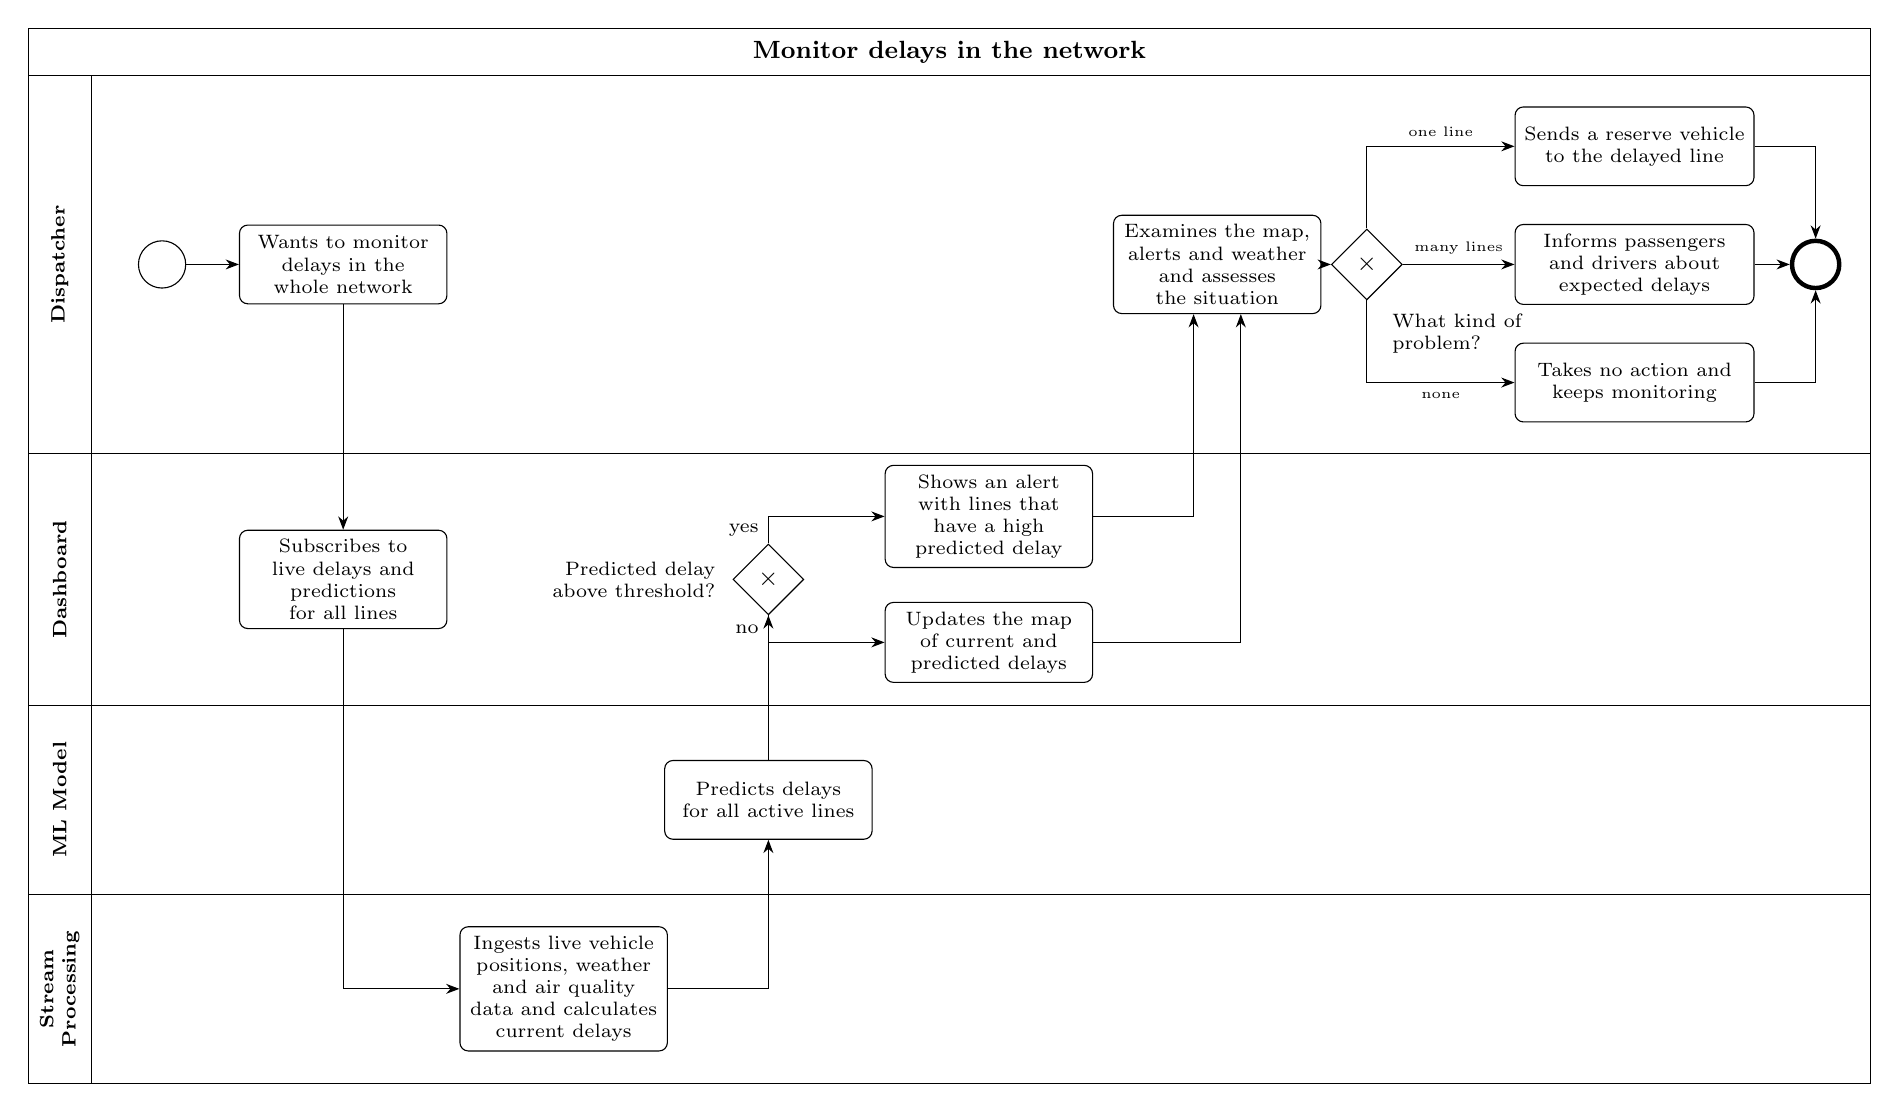
\begin{tikzpicture}[
    task/.style={draw, rounded corners=3pt, text width=2.4cm, minimum height=1cm, align=center, font=\scriptsize, fill=white},
    choice/.style={task, text width=2.8cm},
    event/.style={draw, circle, minimum size=0.6cm, inner sep=0pt, fill=white},
    endevent/.style={event, line width=1.6pt},
    gateway/.style={draw, diamond, minimum size=0.9cm, inner sep=0pt, fill=white, font=\small},
    flow/.style={-{Stealth}, thin},
    lane/.style={font=\scriptsize\bfseries, rotate=90}
]
    % pool and lanes
    \draw (0,0) rectangle (23.4,13.4);
    \draw (0,12.8) -- (23.4,12.8);
    \node[font=\small\bfseries] at (11.7,13.1) {Monitor delays in the network};
    \draw (0.8,0) -- (0.8,12.8);
    \foreach \y in {2.4,4.8,8.0} \draw (0,\y) -- (23.4,\y);
    \node[lane] at (0.4,10.4) {Dispatcher};
    \node[lane] at (0.4,6.4) {Dashboard};
    \node[lane] at (0.4,3.6) {ML Model};
    \node[lane, align=center] at (0.4,1.2) {Stream\\Processing};

    % elements
    \node[event] (s) at (1.7,10.4) {};
    \node[task] (d1) at (4,10.4) {Wants to monitor delays in the whole network};
    \node[task] (d2) at (4,6.4) {Subscribes to live delays and predictions for all lines};
    \node[task] (d3) at (6.8,1.2) {Ingests live vehicle positions, weather and air quality data and calculates current delays};
    \node[task] (d4) at (9.4,3.6) {Predicts delays for all active lines};
    \node[gateway] (g) at (9.4,6.4) {$\times$};
    \node[font=\scriptsize, align=right, anchor=east] at (8.85,6.4) {Predicted delay\\above threshold?};
    \node[task] (d5) at (12.2,7.2) {Shows an alert with lines that have a high predicted delay};
    \node[task] (d6) at (12.2,5.6) {Updates the map of current and predicted delays};
    \node[task] (d7) at (15.1,10.4) {Examines the map, alerts and weather and assesses the situation};
    \node[gateway] (g2) at (17,10.4) {$\times$};
    \node[font=\scriptsize, align=left, anchor=north west] at (17.2,9.9) {What kind of\\problem?};
    \node[choice] (d8) at (20.4,11.9) {Sends a reserve vehicle to the delayed line};
    \node[choice] (d9) at (20.4,10.4) {Informs passengers and drivers about expected delays};
    \node[choice] (d10) at (20.4,8.9) {Takes no action and keeps monitoring};
    \node[endevent] (e) at (22.7,10.4) {};

    % flows
    \draw[flow] (s) -- (d1);
    \draw[flow] (d1) -- (d2);
    \draw[flow] (d2.south) |- (d3.west);
    \draw[flow] (d3.east) -| (d4.south);
    \draw[flow] (d4) -- (g);
    \draw[flow] (g.north) |- node[pos=0.25, left, font=\scriptsize] {yes} (d5.west);
    \draw[flow] (g.south) |- node[pos=0.25, left, font=\scriptsize] {no} (d6.west);
    \draw[flow] (d5.east) -| ([xshift=-3mm]d7.south);
    \draw[flow] (d6.east) -| ([xshift=3mm]d7.south);
    \draw[flow] (d7) -- (g2);
    \draw[flow] (g2.north) |- node[pos=0.75, above, font=\tiny] {one line} (d8.west);
    \draw[flow] (g2.east) -- node[above, font=\tiny] {many lines} (d9.west);
    \draw[flow] (g2.south) |- node[pos=0.75, below, font=\tiny] {none} (d10.west);
    \draw[flow] (d8.east) -| (e.north);
    \draw[flow] (d9) -- (e);
    \draw[flow] (d10.east) -| (e.south);
\end{tikzpicture}%
}
\caption{Business process: dispatcher monitors delays in the network}
\label{fig:bp_dispatcher}
\end{figure}

\FloatBarrier
% \subsection{Benefits for the users}

% \textbf{Passengers} will be able to plan their trips better. Instead of only seeing the timetable, they will know the current and the expected delay of their line, and they will see when bad weather is likely to make travel longer. This can help them decide to leave home earlier or choose a different line.

% \textbf{Dispatchers} will get one place where they can see the whole network, current delays and predicted problems. Thanks to the predictions and alerts they can react earlier, for example by sending an additional vehicle or informing passengers, instead of reacting only after the delay has already grown.

% \textbf{Transport planners and analysts} will get access to historical data that is already cleaned and combined with weather data. This makes it possible to find lines and stops which are regularly late or which are especially affected by bad weather, and to use this knowledge when planning timetables, for example by adding extra time on some routes during winter.

\section{Description of Datasets}
\label{sec:data-sets}

This section describes the data sets used in the project: three streams
(vehicle positions, weather and air quality) and one batch data set
(the GTFS timetable). All numbers were computed with Spark on the data
stored in HDFS, collected between 15 and 22 November 2026.

Because of hardware problems and restarts of our infrastructure, data is
available for about 152 of the 165 hours of this period. For this reason
daily averages were computed only on days with complete data
(18, 19 and 20 November).

\subsection{Vehicle positions (GPS)}

Vehicle positions are the main data source of the project.
Every snapshot contains the current position of every bus and tram in Warsaw together with the GTFS trip it serves,
so each position can be matched with the timetable.
The data is published by Mikołaj Kuranowski on mkuran.pl and is built from the official ZTM data.

\begin{table}[H]
\centering
\caption{Vehicle positions data set.}\label{tab:ds-gps}
\begin{tabular}{|>{\raggedright\arraybackslash}p{3cm}|>{\raggedright\arraybackslash}p{11cm}|}
\hline
\textbf{Property} & \textbf{Description} \\
\hline
Data category & Live GPS positions of buses and trams in Warsaw \\ \hline
Source & \texttt{https://mkuran.pl/gtfs/warsaw/positions.json} \\ \hline
Source format & JSON \\ \hline
Inflow frequency & Polled every 10 s (about 8600 snapshots per day), but updated every 20s \\ \hline
Number of records & On average 812 vehicles per snapshot (about 110 at night, 1070 during the day), about 5.15 million rows per day after cleaning \\ \hline
Volume & About 285 KB per snapshot, 2.46 GB of raw JSON per day \\ \hline
\end{tabular}
\end{table}

\begin{table}[H]
\centering
\caption{Structure of a GPS record.}\label{tab:fields-gps}
\begin{tabular}{|>{\raggedright\arraybackslash}p{3.6cm}|>{\raggedright\arraybackslash}p{2cm}|>{\raggedright\arraybackslash}p{8cm}|}
\hline
\textbf{Field name} & \textbf{Type} & \textbf{Description} \\
\hline
id & String & Unique id of the record \\ \hline
trip\_id & String & GTFS trip served by the vehicle. Used to get the line number and vehicle type from GTFS \\ \hline
side\_number & String & Vehicle (fleet) number \\ \hline
service\_date & String & GTFS service day (YYYYMMDD) \\ \hline
timestamp & Timestamp & Time of the GPS fix (ISO 8601 with time zone offset) \\ \hline
lat, lon & Number & Position of the vehicle (WGS84) \\ \hline
bearing & Number & Direction of movement in degrees (-180 to 180, changed to 0-360 in cleaning) \\ \hline
\end{tabular}
\end{table}

\noindent\textbf{Data quality assessment:}
The data is complete, only \texttt{bearing} is missing in 3.4\% of records. All trip ids were found in GTFS, so every position can be matched with the timetable.
It turned out that about half of the raw records are duplicates - this could mean that we ask the API more often than the data changes. 
Duplicates are removed in cleaning. About 3\% of consecutive positions give a speed above 120 km/h (GPS jumps), so they are filtered out when computing speed features.

\subsection{Weather}

Weather data comes from the city weather stations, which measure air and road temperature, humidity, wind and precipitation.
The measurements are updated only about every 10 minutes, which is too rare to treat them as a real stream.
Because of that the simulator interpolates the values between two measurements and sends a new snapshot every 30 s.
GPS data is buffered for 15 minutes, so that all streams stay synchronised.

\begin{table}[H]
\centering
\caption{Weather data set.}\label{tab:ds-weather}
\begin{tabular}{|>{\raggedright\arraybackslash}p{3cm}|>{\raggedright\arraybackslash}p{11cm}|}
\hline
\textbf{Property} & \textbf{Description} \\
\hline
Data category & Weather measurements from city weather stations in Warsaw \\ \hline
Source & Warsaw open data API (\texttt{dane.um.warszawa.pl}) \\ \hline
Source format & JSON \\ \hline
Inflow frequency & Values change about every 10 minutes, the simulator sends an interpolated snapshot every 30 s (2880 per day) \\ \hline
Number of records & 16 stations per snapshot, 46080 rows per day \\ \hline
Volume & About 3.5 KB per snapshot, 10 MB of raw JSON per day \\ \hline
\end{tabular}
\end{table}

\begin{table}[H]
\centering
\caption{Structure of a weather record.}\label{tab:fields-weather}
\begin{tabular}{|>{\raggedright\arraybackslash}p{3.6cm}|>{\raggedright\arraybackslash}p{2cm}|>{\raggedright\arraybackslash}p{8cm}|}
\hline
\textbf{Field name} & \textbf{Type} & \textbf{Description} \\
\hline
lokalizacja & String & Name of the weather station \\ \hline
lat, lon & Number & Position of the station \\ \hline
czas & Timestamp & Time of the measurement (local time, changed to UTC in cleaning) \\ \hline
temp\_pow & Number & Air temperature (C) \\ \hline
temp\_naw & Number & Road surface temperature (C) \\ \hline
wilg\_pow & Number & Relative air humidity (\%) \\ \hline
pred\_wiatru & Number & Wind speed \\ \hline
kier\_wiatru & Number & Wind direction (degrees) \\ \hline
int\_opadu & Number & Precipitation intensity \\ \hline
\end{tabular}
\end{table}

\noindent\textbf{Data quality assessment:}
All 16 stations are present in every snapshot and no record was rejected in cleaning. The provider marks missing values as -32000 (at most 0.19\% of rows per field), so we treat values outside simple ranges as missing. The main limitation is that there are only 16 stations for the whole city and values change every 10 minutes, so we interpolate them in time and give each vehicle the values from the nearest station.

\subsection{Air quality}

Air quality data comes from monitoring stations in Warsaw.
Most of them are low-cost sensors measuring particulate matter and NO2,
many of them also measure temperature, humidity and pressure.
Same as weather, the values are updated about every 10 minutes,
so they are interpolated by the simulator and sent every 30 s together with the other streams.

\begin{table}[H]
\centering
\caption{Air quality data set.}\label{tab:ds-air}
\begin{tabular}{|>{\raggedright\arraybackslash}p{3cm}|>{\raggedright\arraybackslash}p{11cm}|}
\hline
\textbf{Property} & \textbf{Description} \\
\hline
Data category & Air pollution and sensor measurements from monitoring stations in Warsaw \\ \hline
Source & Warsaw open data API (\texttt{dane.um.warszawa.pl}) \\ \hline
Source format & JSON (nested, list of measurements for each station) \\ \hline
Inflow frequency & Same as weather, snapshot every 30 s (2880 per day) \\ \hline
Number of records & 113 stations and 773 measurements per snapshot, about 2.22 million rows per day \\ \hline
Volume & About 139 KB per snapshot, 400 MB of raw JSON per day \\ \hline
\end{tabular}
\end{table}

\begin{table}[H]
\centering
\caption{Structure of an air quality record.}\label{tab:fields-air}
\begin{tabular}{|>{\raggedright\arraybackslash}p{3.6cm}|>{\raggedright\arraybackslash}p{2cm}|>{\raggedright\arraybackslash}p{8cm}|}
\hline
\textbf{Field name} & \textbf{Type} & \textbf{Description} \\
\hline
name & String & Name of the station \\ \hline
lat, lon & Number & Position of the station \\ \hline
address & Object & Address of the station (used to keep only stations in Warsaw) \\ \hline
data & Array & List of measurements of the station, fields below are for one element \\ \hline
param\_code & String & Code of the parameter, e.g. PM10, PM2.5, NO2, T (temperature), H (humidity), P (pressure) \\ \hline
param\_name & String & Full name of the parameter \\ \hline
value & Number & Measured value \\ \hline
unit & String & Unit of the value, e.g. ug/m3 \\ \hline
time & Timestamp & Time of the measurement (local time, changed to UTC in cleaning) \\ \hline
\end{tabular}
\end{table}

\noindent\textbf{Data quality assessment:}
Every snapshot has the same 113 stations and only 0.13\% of records are rejected because of a negative value. PM, NO2, temperature, humidity and pressure are measured by over 100 stations, but O3, CO, benzene and SO2 only by 1 to 9 stations, so they are not very useful as features. There are also some inconsistencies at the source: PM2.5 comes under two codes (PM2.5 and PM25) and the CO values of the two stations differ a lot, probably because of a wrong unit.

\subsection{Timetable (GTFS)}

The GTFS feed is the static timetable of Warsaw public transport.
It is needed to compute delays, because planned times from the timetable are compared with the real positions of vehicles.
The feed is downloaded once a day, because the timetable changes often.

\begin{table}[H]
\centering
\caption{Timetable (GTFS) data set.}\label{tab:ds-gtfs}
\begin{tabular}{|>{\raggedright\arraybackslash}p{3cm}|>{\raggedright\arraybackslash}p{11cm}|}
\hline
\textbf{Property} & \textbf{Description} \\
\hline
Data category & Static timetable of Warsaw public transport \\ \hline
Source & \texttt{https://mkuran.pl/gtfs/warsaw.zip} \\ \hline
Source format & ZIP archive with CSV files (GTFS standard) \\ \hline
Inflow frequency & Downloaded once a day \\ \hline
Number of records & 324 routes, 7304 stops, 272002 trips, 7771522 stop times (feed from 22 November) \\ \hline
Volume & About 105 MB per archive \\ \hline
\end{tabular}
\end{table}

\begin{table}[H]
\centering
\caption{Main fields of the GTFS tables used in the project.}\label{tab:fields-gtfs}
\begin{tabular}{|>{\raggedright\arraybackslash}p{3.6cm}|>{\raggedright\arraybackslash}p{2cm}|>{\raggedright\arraybackslash}p{8cm}|}
\hline
\textbf{Field name} & \textbf{Type} & \textbf{Description} \\
\hline
route\_id & String & Id of the route \\ \hline
route\_short\_name & String & Line number shown to passengers, e.g. 175 \\ \hline
route\_type & Integer & Type of vehicle (0 tram, 1 metro, 2 rail, 3 bus) \\ \hline
trip\_id & String & Id of the trip, the same as in the GPS data \\ \hline
route\_id & String & Route of the trip \\ \hline
service\_id & String & Days on which the trip runs (see calendar\_dates) \\ \hline
direction\_id & Integer & Direction of the trip (0 or 1) \\ \hline
stop\_id & String & Id of the stop \\ \hline
stop\_name & String & Name of the stop \\ \hline
stop\_lat, stop\_lon & Number & Position of the stop \\ \hline
trip\_id & String & Trip that the stop time belongs to \\ \hline
stop\_sequence & Integer & Order of the stop in the trip \\ \hline
stop\_id & String & Stop \\ \hline
arrival\_time, departure\_time & String & Planned times (HH:MM:SS, can be after 24:00 for night services) \\ \hline
service\_id & String & Id of the service \\ \hline
date & String & Date (YYYYMMDD) \\ \hline
exception\_type & Integer & 1 if the service runs on this date, 2 if not \\ \hline
\end{tabular}
\end{table}

\noindent\textbf{Data quality assessment:}
The GTFS data is complete and well structured, but it changes almost every day (6 out of 7 downloaded feeds are different),
so we always use the feed that was valid on the day of the observation. 
About 3\% of stop times are later than 24:00, which is normal in GTFS for night services, so we convert them to seconds from the start of the service day.
The feed from 17 November is missing because of our infrastructure outage, in that case the previous feed is used since it covers the next month anyway.

\subsection{Conceptual Data Model}

The conceptual data model of the system is presented in Figure~\ref{fig:conceptual-model}.
It consists of four entities, one for each data source:

\begin{itemize}
    \item \textbf{Vehicle Positions} -- live GPS positions of active buses and trams,
    including trip id, vehicle number and timestamp.
    \item \textbf{Timetables} -- planned stop times of every trip, together with routes
    and stop locations, downloaded once per day.
    \item \textbf{Weather Observations} -- meteorological conditions (temperature,
    precipitation, humidity, wind) measured at stations across the city.
    \item \textbf{Air Quality Observations} -- air quality parameters measured at
    monitoring stations across the city.
\end{itemize}

Vehicle Positions is the central entity. It is associated with Timetables via trip id, stop and time, which allows the delay of a vehicle to be calculated. It is also
associated with Weather Observations and Air Quality Observations via time and location,
which allows delays to be related to the conditions in which they occurred. Timetables
remain a separate entity because, unlike the other entities, they come from a daily batch
source rather than a stream.

\begin{figure}[htbp]
    \centering
    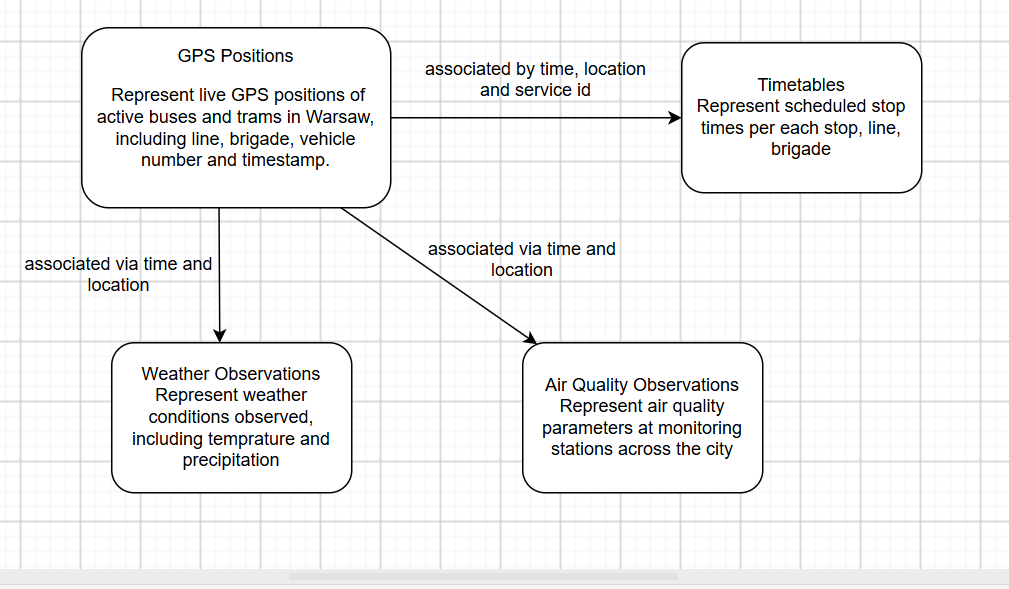
\includegraphics[width=\textwidth]{conceptual_data_model.png}
    \caption{Conceptual data model illustrating relationships between source datasets
    using temporal and spatial associations.}
    \label{fig:conceptual-model}
\end{figure}

\subsection{Machine-learning data set (\texttt{ml\_dataset})}

The ML data set is saved as Parquet and partitioned by date (UTC). It has 44 columns and one row per vehicle, trip and minute.
Each row describes one vehicle: its position, its delay history, the weather and air quality from the nearest stations in the same minute
and the delay it will have about 10 minutes later. Table~\ref{tab:ml} shows the columns grouped by their role.

\begin{table}[H]
\centering
\small
\caption{Columns of the ML data set.}\label{tab:ml}
\begin{tabular}{|>{\raggedright\arraybackslash}p{2.4cm}|>{\raggedright\arraybackslash}p{4.4cm}|>{\raggedright\arraybackslash}p{6.6cm}|}
\hline
\textbf{Role} & \textbf{Columns} & \textbf{Description} \\
\hline
Row key (not features) & event\_time\_utc, trip\_id, side\_number, service\_date, date & Identify the row (minute, trip, vehicle) and the partition. Used only for joins and for splitting the data by time \\
\hline
\multicolumn{3}{|l|}{\textit{Independent features (30)}} \\
\hline
Line & route\_short\_name, route\_type, direction\_id & Taken from GTFS using trip\_id. route\_type is 0 for tram and 3 for bus \\
\hline
Position & lat, lon & GPS position \\
\hline
Time & hour\_local, day\_of\_week, is\_weekend, is\_rush\_hour & Computed in Warsaw local time, rush hour is 7-9 and 15-18 on weekdays \\
\hline
Movement & speed\_kmh, speed\_avg\_5min\_kmh & Speed between two pings and its 5-minute average. Empty if the gap is longer than 180 s or the speed is above 120 km/h \\
\hline
Delay history & last\_delay\_s, last\_delay\_age\_s, delay\_change\_s & Delay at the last stop of the same vehicle (at least 30 s before the row), how old it is and how it changed since the previous stop \\
\hline
Trip progress & last\_stop\_sequence, trip\_last\_sequence, trip\_progress & How far the vehicle is in its trip, trip\_progress is from 0 to 1 \\
\hline
Weather & temp\_air, temp\_road, humidity, wind\_speed, wind\_dir\_sin, wind\_dir\_cos, precip\_intensity, is\_raining, weather\_missing & Values from the nearest weather station in the same minute. Wrong values are set to empty, wind direction is saved as sine and cosine \\
\hline
Air quality & air\_pm10, air\_pm2\_5, air\_no2, air\_missing & Values from the nearest station that measures the parameter, in the same minute \\
\hline
Not used as features & route\_id, wind\_dir, weather\_station\_dist\_m, air\_pm10\_dist\_m, air\_pm2\_5\_dist\_m, air\_no2\_dist\_m & Replaced by other columns (sine and cosine) or only show the distance to the station that was used \\
\hline
\multicolumn{3}{|l|}{\textit{Dependent variable}} \\
\hline
Target & target\_delay\_s & Delay in seconds at the first stop visited at least 10 minutes after the row \\
\hline
Target helpers & target\_horizon\_s, has\_target & Real time to the target stop (600-900 s) and a flag if the row has a target. target\_horizon\_s is not a feature, because it is not known when predicting \\
\hline
\end{tabular}
\end{table}

\noindent\textbf{Transformations.}
First, stop visits and delays are estimated from the GPS pings and the timetable of the matching GTFS feed. The delay is the time
when the vehicle was at the stop minus the planned departure time, so a positive value means the vehicle is late.
Then each ping gets the weather and air quality values from the nearest station in the same minute (the nearest stations are
computed once for a grid of cells). After that the time, speed, trip progress and delay history features are computed.
At the end the target is added by looking at later stops of the same trip: we take the first stop at least 600 s ahead,
if it is reached within 900 s.

\noindent\textbf{Missing targets and values.}
Rows from the last minutes cannot have a target yet, so they have has\_target set to false. The data set is rebuilt at most every
12 hours for the last two days, and then the missing targets are filled. Rows without a stop 10-15 minutes ahead (end of a trip,
missing pings) also have no target and are not used for training. Movement, weather and air quality values can be empty, the
\texttt{*\_missing} flags are kept as features.

\section{Data Processing Steps}

The proposed solution is based on the Lambda Architecture, which combines the processing of current observations with the analysis of historical data. These paths support real-time delay predictions and historical statistics. Their results are brought together in a serving layer and displayed through a dashboard. Figure~\ref{fig:lambda-data-flow} presents the overall data flow.

\begin{figure}[H]
    \centering
    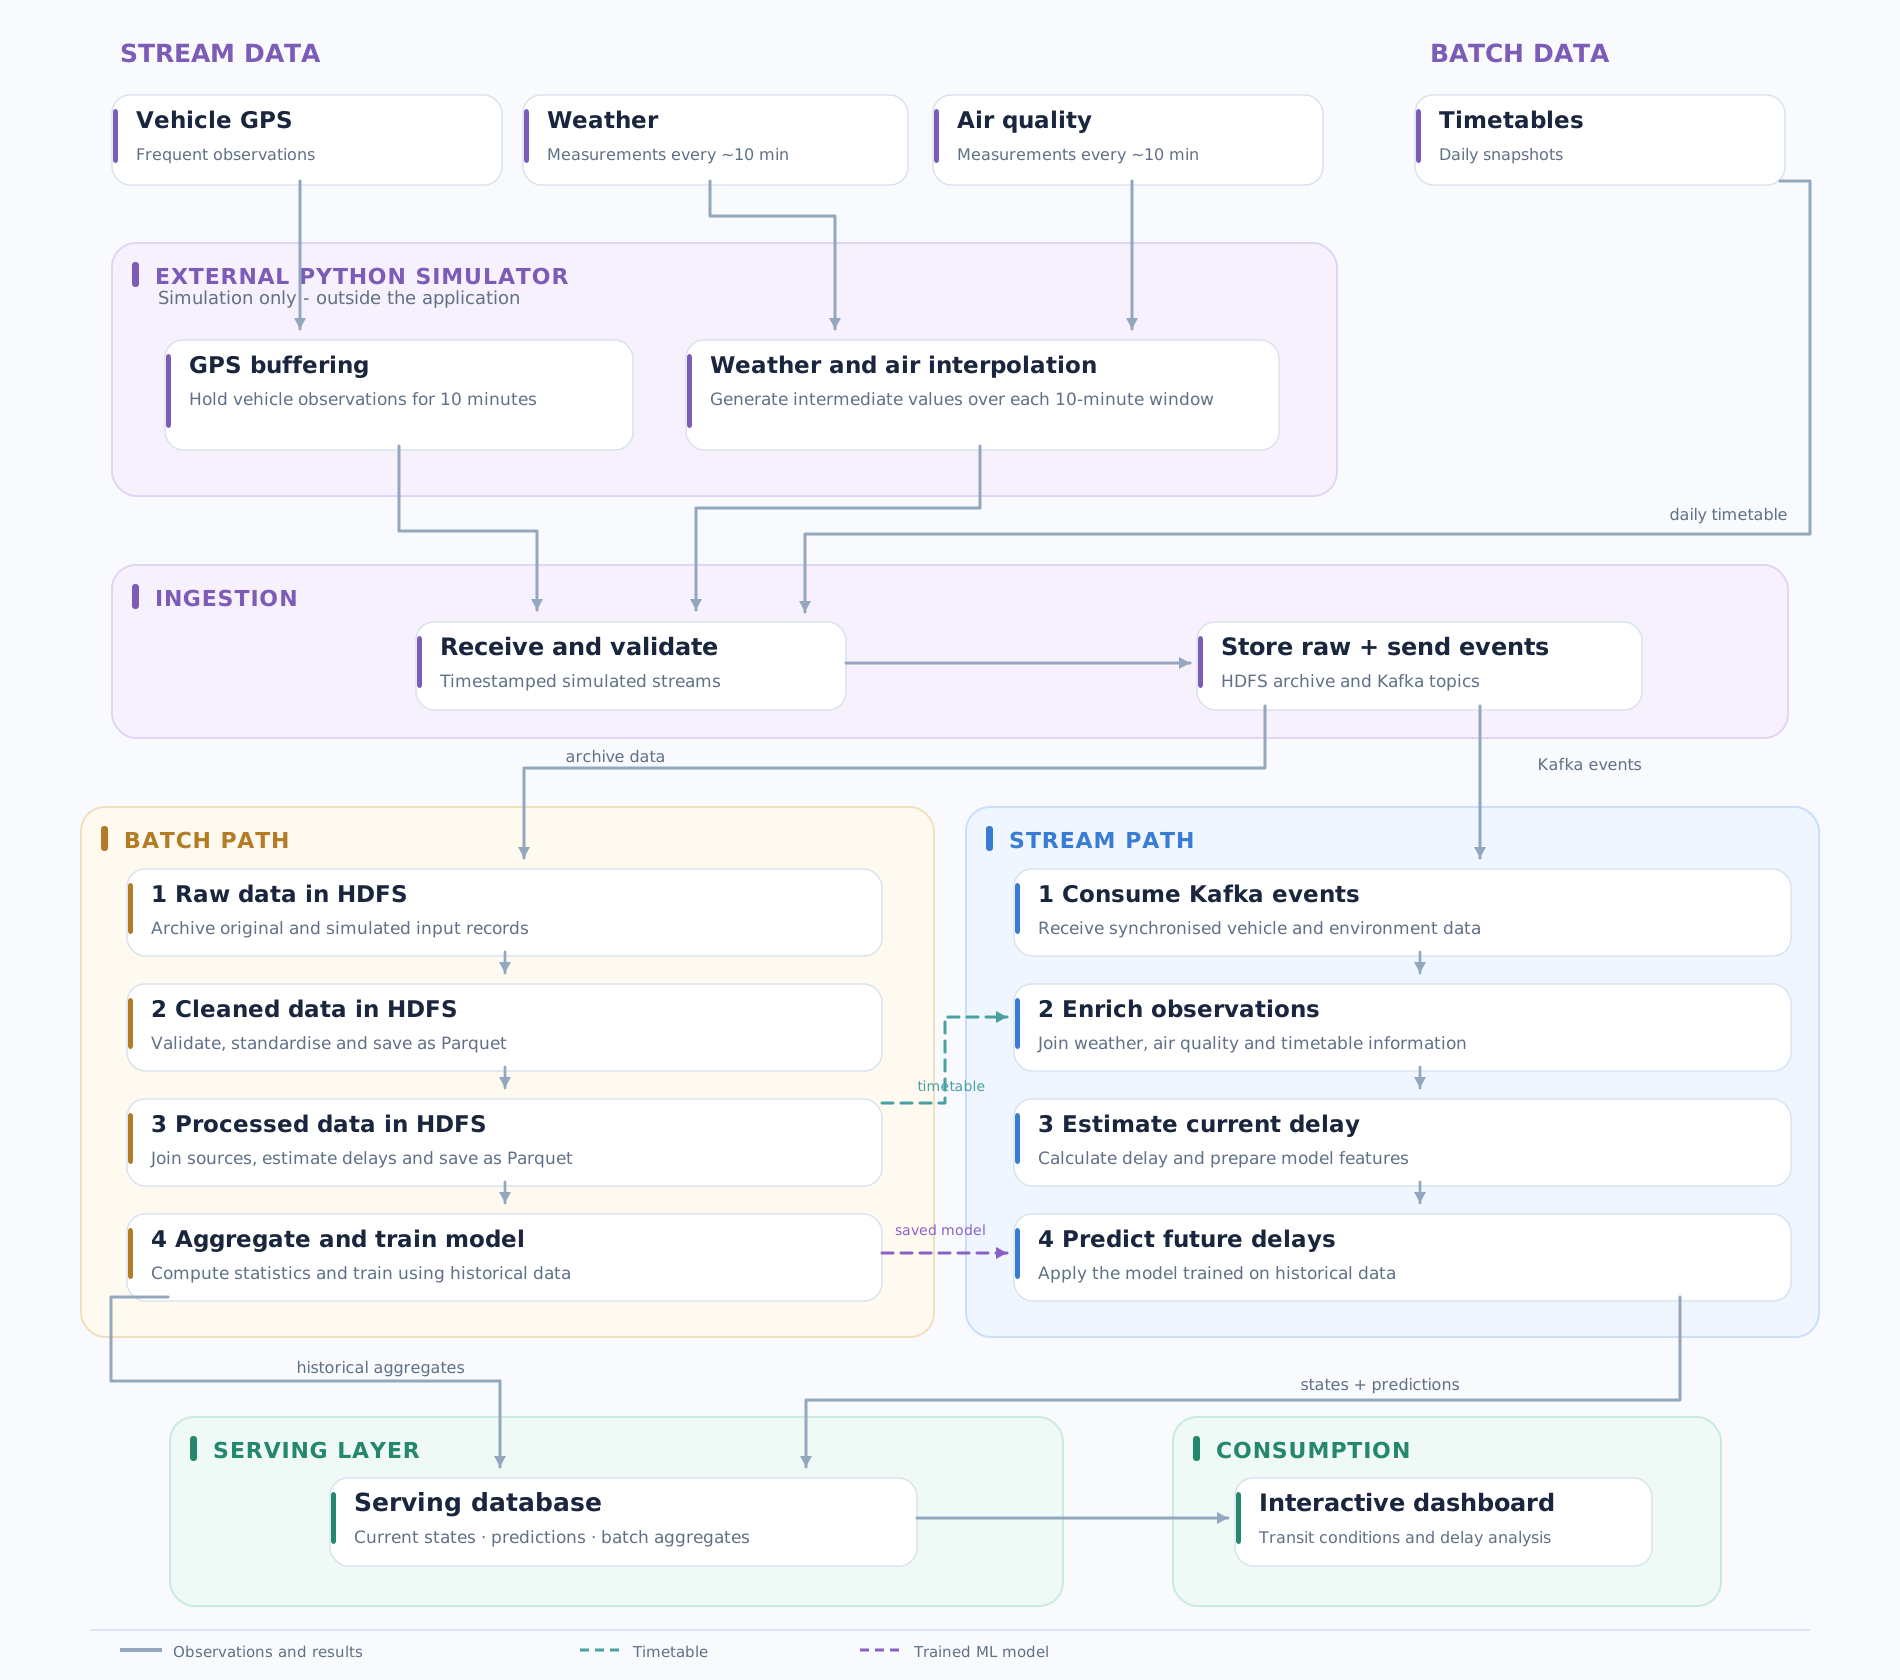
\includegraphics[width=\linewidth,height=0.8\textheight,keepaspectratio]{lambda_data_flow.png}
    \caption{High-level data flow for stream and batch processing.}
    \label{fig:lambda-data-flow}
\end{figure}

\subsection{Data Ingestion}

The system will collect three types of stream data: vehicle GPS positions, weather measurements, and air quality measurements. Public transport timetables will form a separate batch source, refreshed approximately once per day. A separate Python module will buffer GPS observations for 15 minutes and interpolate weather and air quality measurements within the corresponding windows. It will send synchronised streams to the ingestion component, while timetable data will be retrieved separately. The ingestion component will validate incoming data and store raw records in HDFS. GPS and environmental observations will also be forwarded to Kafka for stream processing.

\subsection{Batch Processing}

The batch path will use historical data stored in HDFS. The data will be organised into three groups. Raw will contain the original source records. Cleaned will contain validated and standardised data. Processed will contain integrated datasets, estimated delays, and features prepared for further analysis. Apache Spark will perform the cleaning and processing steps, saving both the cleaned and processed datasets in HDFS in Parquet format.

Historical GPS observations will be combined with timetables and environmental measurements to estimate delays. Spark will then calculate statistics such as average delays by line, stop, time period, and weather conditions. Historical datasets and aggregates will be retained in HDFS, while selected statistics will also be written to Cassandra for the dashboard.

A prediction model will be trained and evaluated using the processed historical data. The trained model will be stored in HDFS for use by the stream path. The batch path will also provide the latest processed timetable for real-time calculations.

\subsection{Stream Processing}

The stream path will receive synchronised GPS, weather, and air quality events from Kafka. Current vehicle positions will be combined with environmental measurements and the latest processed timetable. The system will estimate current delays, prepare model features, and use the model trained in the batch path to predict future delays.

Current vehicle positions, environmental measurements, estimated delays, predictions, and real-time statistics will be written to Cassandra.

\subsection{Data Consumption}

The Streamlit dashboard will read current information and historical aggregates from Cassandra. Users will be able to view vehicle positions, environmental conditions, historical delay patterns, and delay predictions in one application.

\section{Solution Architecture}

The system will use open-source Big Data technologies organised into ingestion, batch, speed, serving, and consumption components. The solution will be deployed using Docker Compose, with the main components running in containers to simplify setup and integration. Figure~\ref{fig:lambda-architecture} shows the proposed technologies and their main connections.

\begin{figure}[H]
    \centering
    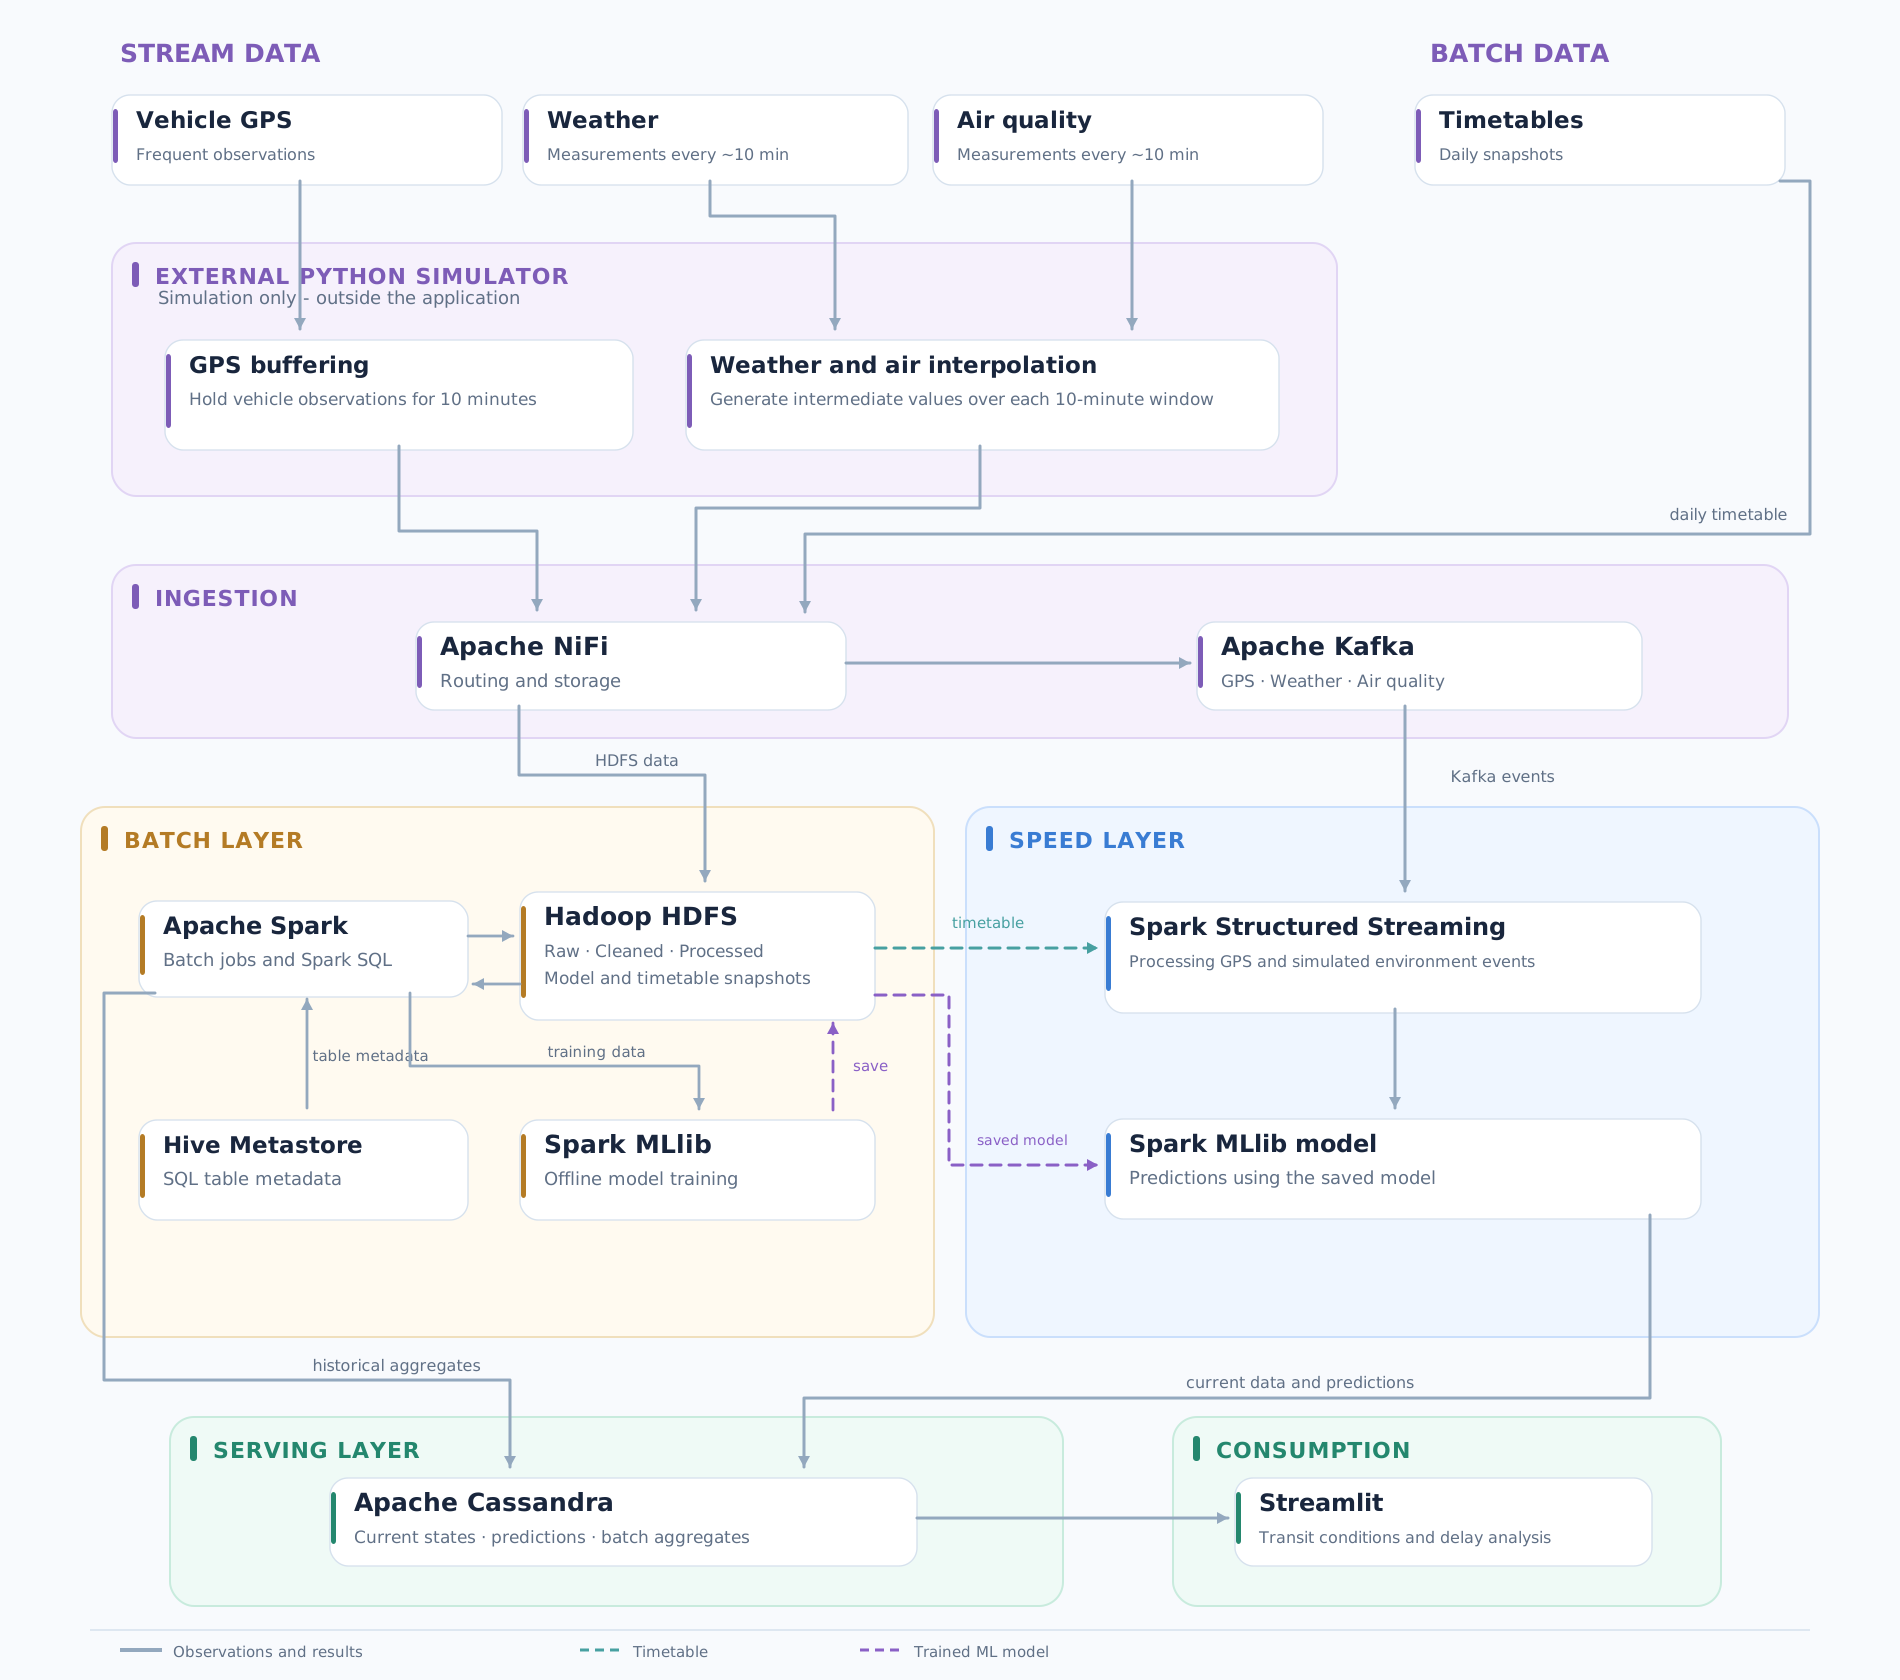
\includegraphics[width=\linewidth,height=0.8\textheight,keepaspectratio]{lambda_architecture.png}
    \caption{Proposed technology architecture based on the Lambda model.}
    \label{fig:lambda-architecture}
\end{figure}

\subsection{Ingestion Layer}

A separate \textbf{Python simulation module} will buffer GPS observations for 15 minutes and interpolate weather and air quality measurements to create synchronised streams. The module will run before NiFi and outside the main application. \textbf{Apache NiFi} will receive the simulated streams and retrieve daily timetables. It will save raw observations and timetables in HDFS and forward GPS, weather, and air quality events to \textbf{Apache Kafka}. Kafka will organise the incoming records into separate topics for the stream processing application.

\subsection{Batch Layer}

\textbf{Hadoop HDFS} will store raw, cleaned, and processed data, as well as timetable snapshots and trained models. \textbf{Apache Spark} will clean and combine historical records, prepare datasets, and calculate aggregates. \textbf{Hive Metastore} will maintain table definitions for datasets stored in HDFS, allowing them to be accessed through Spark SQL.

\textbf{Spark MLlib} will be used to train and evaluate the delay prediction model. The model will be saved in HDFS and made available to the speed layer.

\subsection{Speed Layer}

\textbf{Apache Spark Structured Streaming} will read events from Kafka and process current observations. It will use the latest timetable and the trained \textbf{Spark MLlib} model to calculate delays and generate predictions. Current observations, statistics, and predictions will be saved to Cassandra.

\subsection{Serving Layer and Dashboard}

\textbf{Apache Cassandra} will store current information from the speed layer and selected historical aggregates and model evaluation metrics from the batch layer. \textbf{Streamlit} will provide a dashboard that reads these results from Cassandra and presents them through interactive visualisations.

\section{Analytical Approach}
\label{sec:analytics}

\subsection{Tasks}

\begin{table}[H]
\centering
\small
\caption{Analytical tasks, processing mode and status.}\label{tab:tasks}
\begin{tabular}{|>{\raggedright\arraybackslash}p{3.1cm}|>{\raggedright\arraybackslash}p{2.2cm}|>{\raggedright\arraybackslash}p{2.3cm}|>{\raggedright\arraybackslash}p{2.4cm}|>{\raggedright\arraybackslash}p{2.5cm}|}
\hline
\textbf{Task} & \textbf{Type} & \textbf{Layer} & \textbf{Data} & \textbf{Status} \\
\hline
Delay of each vehicle at stops & Descriptive & Batch (history), stream (current) & stop\_visits, schedule\_stops & Batch implemented, stream planned \\
\hline
Delay prediction about 10 minutes ahead & Regression & Batch training, stream prediction & ml\_dataset & Data set and baselines implemented, model planned \\
\hline
Alerts for lines and areas with high predicted delay & Threshold on predictions & Stream & Model output & Planned \\
\hline
Historical delay statistics by line, stop, hour, weekday and weather & Aggregation & Batch & stop\_visits, ml\_dataset & Planned \\
\hline
Weather impact (dry vs rainy days, most weather-sensitive lines and stops) & Comparison and correlation & Batch & ml\_dataset & Planned \\
\hline
Reference models (no change, predict zero) & Baselines & Batch & ml\_dataset & Implemented \\
\hline
\end{tabular}
\end{table}

\subsection{Delay prediction}

The task is a regression of target\_delay\_s, which is the delay of a vehicle at the first stop visited 10-15 minutes after
the current time. It is predicted from the 30 independent features from Table~\ref{tab:ml}. Only rows with a target are used.
Features that are not known in real time (like target\_horizon\_s) are not used, so the same model can later be used in the
speed layer.

We plan to use linear regression from Spark MLlib as a simple reference and gradient-boosted trees as the main model.
The best model will be saved in HDFS for the speed layer.

The models will be evaluated with MAE and RMSE. The data will be split by time: earlier days for training and the latest days
for testing, so that no information from the future gets into training. The model has to beat two baselines: no change
(prediction equals last\_delay\_s) and predict zero (the vehicle is on time). The MAE of both baselines is already computed
for every build of the data set.

\subsection{Historical statistics and weather impact}

Batch jobs will compute average delays by line, stop, hour, day of the week and weather. They will also compare delays on dry
and rainy days (and in other conditions like strong wind or low temperature) and rank the lines and stops whose delays grow the
most in bad weather.

\subsection{Batch and stream}

\begin{table}[H]
\centering
\small
\caption{Processing mode of each result.}\label{tab:mode}
\begin{tabular}{|>{\raggedright\arraybackslash}p{4cm}|>{\raggedright\arraybackslash}p{1.8cm}|>{\raggedright\arraybackslash}p{7.6cm}|}
\hline
\textbf{Result} & \textbf{Mode} & \textbf{Reason} \\
\hline
Model training and evaluation & Batch & Needs the whole history, a delay of a few hours is not a problem \\
\hline
Historical statistics, weather ranking & Batch & Aggregation over all collected days \\
\hline
Current delay of each vehicle & Stream & Computed from live pings and the timetable, with the same delay definition as in batch \\
\hline
Delay prediction and alerts & Stream & Features computed from live data and scored with the model trained in batch \\
\hline
\end{tabular}
\end{table}

All sources are delayed by 15 minutes by the simulator, so the stream shows the situation from 15 minutes earlier.

\subsection{Presentation of results to end users}

The results will be shown in a Streamlit dashboard for passengers, operators and analysts. Live panels read data from
Cassandra, historical panels read batch aggregates that are also exported to Cassandra. The dashboard will have:
\begin{itemize}
  \item a map with vehicles coloured by their current delay, filters by line and stop, and current weather and air quality,
  \item predicted delays for the selected line and a list of lines and areas where the predicted delay is above a chosen threshold,
  \item historical statistics, average delays by line, stop, hour, day of the week and weather,
  \item a ranking of lines and stops most sensitive to bad weather,
  \item model quality metrics compared with the baselines.
\end{itemize}

\section{Use of Artificial Intelligence}

AI tools will be used throughout the project to support software development, technical problem-solving, and report preparation. Their use will focus on improving productivity and assisting the team while ensuring that \textbf{all generated content and code are reviewed and verified by the team members}. \\ \\
The planned uses of AI include:
\begin{itemize}
    \item \textbf{Code development and editing:} Using AI tools integrated into the IDE to assist with writing, editing and debugging the code.
    \item \textbf{Technical support:} Using AI to clarify technical concepts, explain unfamiliar technologies, suggest implementation approaches, and assist in troubleshooting errors.
    \item \textbf{Report writing and editing:} Using AI to help structure the report, improve clarity and readability, correct grammatical and linguistic errors, and refine technical descriptions.
    \item \textbf{Verification of results:} Reviewing and testing AI-generated code, suggestions, and written content to ensure their correctness, relevance, and consistency with the actual project implementation.
\end{itemize}
AI will serve as a supporting tool rather than a replacement for the team's own work. All team members will remain responsible for understanding, validating, and maintaining the code and documentation they produce.

\section{Division of Responsibilities}

\begin{table}[H]
\centering
\small
\caption{Distribution of responsibilities among team members}
\label{tab:responsibilities}
\begin{tabular}{>{\raggedright\arraybackslash}p{7.2cm} c c c c}
\toprule
\textbf{Responsibility} & \textbf{Emil} & \textbf{Michał} & \textbf{Sebastian} & \textbf{Tymoteusz} \\
\midrule
1. API access, Python stream simulation and Apache NiFi ingestion
   &  & \mainresp & \suppresp &  \\
2. Kafka topics and data validation
   &  & \mainresp & \suppresp &  \\
3. Data schemas and interfaces (HDFS paths, Kafka topics, Cassandra tables)
   & \suppresp & \suppresp & \mainresp & \suppresp \\
4. HDFS, directory structure and data cleaning (Parquet)
   & \mainresp & \suppresp &  &  \\
5. Delay estimation and feature definitions shared by batch and stream paths
   & \mainresp &  &  & \suppresp \\
6. Batch processing: unified dataset, historical statistics and weather-sensitivity ranking
   & \mainresp & \suppresp &  &  \\
7. ML model training, evaluation and saving the model in HDFS
   & \mainresp &  &  & \suppresp \\
8. Spark Structured Streaming: Kafka consumption, enrichment, live delays and predictions
   & \suppresp &  &  & \mainresp \\
9. Live delays and predictions
   & \suppresp &  &  & \mainresp \\
10. Cassandra tables and writing/exporting results from batch and stream processing
   & \suppresp &  & \mainresp & \suppresp \\
11. Streamlit dashboard (map, alerts, weather impact analysis, model quality)
   &  &  & \mainresp & \suppresp \\
12. Docker Compose integration, system testing and run documentation
   & \suppresp & \suppresp & \mainresp & \suppresp \\
\bottomrule
\end{tabular}

\vspace{2mm}
\footnotesize
{\Large$\checkmark$} -- main responsible person, \quad {\footnotesize$\checkmark$} -- supporting team member
\end{table}

The project work is divided among four team members, each responsible for a specific component of the system and supported by another team member.

\subsection{Data Ingestion and Validation}

\textbf{Main responsible person:} Michał, \textbf{supporting team member:} Sebastian.

\begin{itemize}
    \item Selecting and testing data sources for vehicle positions and timetables (mkuran.pl) and for weather and air quality (Warsaw open data API).
    \item Creating scripts in order to retrieve data from external APIs.
    \item Implementing a Python simulation module for 15-minute GPS buffering and interpolation of weather and air quality measurements.
    \item Configuring Apache NiFi to automate the data ingestion process, including daily retrieval of timetables.
    \item Storing raw copies of all collected data in HDFS (Raw layer).
    \item Configuring Apache Kafka topics, such as \texttt{gps}, \texttt{weather} and \texttt{air\_quality}.
    \item Implementing data validation, error handling and duplicate detection.
    \item Defining and documenting data schemas.
    \item Documenting the data collection process.
\end{itemize}
\textbf{Expected outcome:} A working data ingestion pipeline that retrieves and validates data, archives raw data in HDFS and delivers live data to Apache Kafka, with a separate Python module for buffering GPS observations and interpolating weather and air quality measurements.

\subsection{Data Storage and Batch Processing}

\textbf{Main responsible person:} Emil, \textbf{supporting team member:} Michał.

\begin{itemize}
    \item Configuring Apache Hadoop and HDFS.
    \item Designing a directory structure for raw, cleaned and enriched data, timetable snapshots and trained models.
    \item Cleaning the collected data and handling missing or invalid values, and saving it in Parquet format.
    \item Estimating historical delays of buses and trams by comparing GPS positions with timetables, using delay logic shared with the stream path.
    \item Combining GPS, timetable, weather and air quality data into a unified dataset, including features for machine learning, with feature definitions shared with the stream path.
    \item Implementing batch processing jobs using Apache Spark.
    \item Calculating historical statistics, such as average delays of buses and trams by line, stop, hour, day of the week and weather conditions, including a ranking of weather-sensitive lines and stops.
    \item Training a Spark MLlib model that predicts delays of buses and trams, using the enriched dataset.
    \item Evaluating the model with metrics and saving the trained model in HDFS for the stream path.
    \item Publishing the latest timetable snapshot in HDFS for the stream path.
    \item Exporting historical aggregates and model evaluation metrics to Cassandra.
\end{itemize}
\textbf{Expected outcome:} A functional data storage layer, a unified dataset with estimated delays and features, a repeatable batch processing pipeline for historical analysis, a trained and evaluated prediction model, and aggregates, metrics, model and timetable snapshot delivered to the serving and stream layers.

\subsection{Stream Processing and Prediction}

\textbf{Main responsible person:} Tymoteusz, \textbf{supporting team member:} Emil.

\begin{itemize}
    \item Configuring Apache Spark Structured Streaming.
    \item Implementing the consumption of events from Apache Kafka.
    \item Enriching live observations with the latest weather and air quality data and the timetable snapshot from the batch layer.
    \item Calculating real-time metrics and statistics using streaming data, including current delays, with the same delay definition as in the batch path.
    \item Preparing features from weather, air quality and public transport data, identical to the features used for model training.
    \item Loading the trained model from HDFS and integrating it into the streaming pipeline to generate delay predictions for buses and trams.
    \item Writing current vehicle states, environmental data and predictions to Cassandra.
\end{itemize}
\textbf{Expected outcome:} A working stream processing pipeline capable of calculating real-time metrics and generating bus and tram delay predictions using the model trained in the batch layer.

\subsection{Results Serving, Dashboard, and System Integration}

\textbf{Main responsible person:} Sebastian, \textbf{supporting team member:} Tymoteusz.

\begin{itemize}
    \item Configuring Apache Cassandra and creating tables for current data, predictions, historical aggregates and model metrics.
    \item Defining common data formats and interfaces.
    \item Integrating the results of batch and stream processing.
    \item Developing an interactive dashboard using Streamlit, reading data from Cassandra.
    \item Visualising a map of vehicle delays, weather and air quality conditions, bus and tram delays, historical statistics, weather impact analysis, and machine learning predictions.
    \item Integrating system components using Docker Compose.
    \item Testing the overall system and resolving integration issues.
    \item Preparing instructions for setting up and running the complete system.
\end{itemize}
\textbf{Expected outcome:} A functional dashboard presenting the results of the project, an integrated system running in Docker Compose, and documentation explaining how to run the application.

\end{document}